\documentclass[12pt]{spieman}
\usepackage[T1]{fontenc}
\usepackage[utf8]{inputenc}
\usepackage{amsmath,amssymb,booktabs,array,graphicx,caption,subcaption}
\usepackage{threeparttable,tabularx,adjustbox,enumitem,float,xcolor,lineno}
\hypersetup{colorlinks=true,citecolor=blue,urlcolor=blue,linkcolor=blue}
\ifdefined\pdfminorversion\pdfminorversion=7\fi
\setlength{\emergencystretch}{2em}
\graphicspath{{figures/}}
% Shared mathematical notation.
\newcommand{\IoU}{\mathrm{IoU}}
\newcommand{\mIoU}{\mathrm{mIoU}}
\newcommand{\R}{\mathbb{R}}
\newcommand{\E}{\mathbb{E}}
\newcommand{\indicator}[1]{\mathbb{1}\!\left\{#1\right\}}
\newcommand{\leafset}{\mathcal{C}}
\newcommand{\supportedset}{\mathcal{C}_{\mathrm{sup}}}

% Compatibility name: preserve the audited source citation keys and sentences.
\newcommand{\citep}[1]{\cite{#1}}
\title{Auditing Source-Label Coverage and Recovery--Retention Trade-offs in Cross-Dataset Land-Cover Segmentation}
\author[1]{Yangxi Luo}
\author[2,*]{Liang Cheng}
\author[2]{Jiawen Pan}
\affil[1]{Fuzhou Polytechnic University, Fuzhou, China}
\affil[2]{Fujian Agriculture and Forestry University, Fuzhou, China}
\begin{document}
\maketitle
\linenumbers
\begin{spacing}{2}
\begin{abstract}
A near-zero cross-dataset segmentation score does not, by itself, separate visual domain shift from absence of source annotations assigned to the evaluated output class. We examine this ambiguity through a raw-mask coverage audit and fixed-budget source-mixture experiments under a declared seven-leaf operational crosswalk, with OpenEarthMap rangeland treated as a vegetation proxy whose native scope also includes shrubs. In the primary LoveDA--OpenEarthMap case, adding the tested FLAIR herbaceous source mixture increases rangeland IoU by 0.3118 but decreases mIoU over six LoveDA-supported leaves by 0.1011. A reanalysis of archived native ResNet-34 U-Net records on the same target shows the same direction: rangeland recovery of 0.2828 and supported-leaf mIoU change of -0.1304. A reversed source mixture recovers cropland with another supported-leaf cost, while Semantic Drone supplies a separate target replay of the primary CLIP checkpoints. These results extend established label-space and negative-transfer concerns through a specific audited empirical design; they introduce no new segmentation algorithm or recovery metric. Source mixtures change imagery and labels jointly, and historical checkpoint and schedule provenance remains incomplete. The evidence therefore supports bounded descriptive contrasts rather than a label-only causal effect or a successful mitigation method. Positive source-label coverage, missing-leaf recovery and supported-leaf retention should be reported together.

\end{abstract}
\keywords{land-cover legend harmonization, label coverage, cross-dataset segmentation, OpenEarthMap, FLAIR, vision-language probe, audit protocol}

\par
\noindent Corresponding author: Liang Cheng, \href{mailto:52370034073@fafu.edu.cn}{52370034073@fafu.edu.cn}.

\section{Introduction}
\label{sec:introduction}
Land-cover models are often trained on one mapping product and evaluated on another. Changes in imagery, sensor, resolution and geography can alter performance, while differences in the products' legends change what the learner is positively supervised to recognize \citep{tuia2016domain,bruzzone2009domain,yang2017harmonization}. If a target class is absent from the exact source labels, a near-zero target IoU is difficult to interpret without checking that absence. It is not sufficient evidence that visual domain shift alone caused the failure.

We call the finest software output category used in a mapping decision an \emph{operational leaf}; this is not a claim of a fully reconciled botanical taxonomy. Under a declared crosswalk, a target leaf may have exact source support, only coarse ancestral support, or no mapped support. These are supervision records, not mutually exclusive causes of transfer error. Exact-label absence also does not imply that a pretrained model has no representation of the concept, or that heterogeneous supervision cannot support it. It means that the specified source-training masks supply no positive exact-leaf examples, although the loss can still affect that leaf's predictions.

Label-space reconciliation and annotation conflicts are established concerns: MSeg reconciles taxonomies and pixel annotations, and UniSeg handles multi-dataset label shifts \citep{lambert2020mseg,kim2022uniseg}. Separately reporting common/private performance and examining negative transfer also have precedents \citep{choe2024bus,choe2025unida,ren2026sats}. Our question is narrower: what does a raw-mask support audit reveal about the interpretation of a specific transfer failure, and how much recovery and supported-leaf retention accompany the tested source mixture under fixed update and exposure controls?

LoveDA lacks a raw label assigned to the herbaceous output index in the frozen codebook, whereas FLAIR raw ID 10 supplies that training assignment. OpenEarthMap rangeland is a broader target-label proxy for this index, not a pure herbaceous reference (Supplementary Section S2). The primary CLIP-based experiment compares a LoveDA-only baseline with a LoveDA--FLAIR mixture while retaining the target replay population. Exposure and duplicate-crop controls constrain changes in LoveDA sampling and update representation. An archived native U-Net comparison checks the recovery/retention direction in another recorded model family on the same target. A recorded mismatched image--mask configuration supplies a separate, provenance-limited CLIP sensitivity. Auxiliary imagery and labels enter together, so none of these source-mixture comparisons isolates a label-only causal effect.

The contribution is an empirical audit and diagnostic design within this bounded setting. It connects a versioned operational crosswalk to raw-mask positive support; reports missing-leaf recovery beside source-supported retention under the specified controls; and examines recorded model-family and reversed-source extensions with their distinct dependence and provenance limits. The primary contrast is +0.3118 for rangeland IoU and -0.1011 for supported-leaf mIoU; archived U-Net records repeat the direction. The calibration adapter and U-Net are measurement instruments, not proposed algorithms. We make no first-discovery claim about label mismatch or negative transfer and claim no validated remedy for the observed trade-off.

\section{Related work}
\label{sec:related_work}
\paragraph{Legend harmonization and multi-dataset labels.}
Land-cover harmonization addresses incompatible nomenclatures and mapping scales \citep{yang2017harmonization,baudoux2021translation}. MSeg additionally reconciles pixel annotations across datasets \citep{lambert2020mseg}; UniSeg formulates multi-dataset label conflicts and learns a shared representation \citep{kim2022uniseg}. The HTSS preprint integrates conflicting label spaces and different annotation types through a universal taxonomy \citep{meletis2023htss}. These works preclude treating taxonomy unification or heterogeneous-source learning as new here. Our operational audit records whether a mapped exact label actually occurs in the source masks used by the specified training protocol.

\paragraph{Open-set adaptation and recovery/retention reporting.}
Domain-adaptation methods address changes in representations and output distributions \citep{ganin2016dann,hoffman2018cycada,vu2019advent,zou2018classbalanced}. BUS and UniDA-SS explicitly handle differences between source and target class spaces and evaluate common/private performance \citep{choe2024bus,choe2025unida}. The SATS preprint also identifies known-class negative transfer and unknown-class underfitting \citep{ren2026sats}. Thus, balancing recovery and retention is established framing. The present estimands concern a named added leaf inside a fixed seven-leaf output space, with positive auxiliary-source supervision, rather than claiming a new open-set adaptation method or metric. We measure the tested mixtures' observed gain and cost without claiming superiority over these methods.

\paragraph{Transferable land-cover semantics and non-exact guidance.}
TACOSS uses textual supervision to align visual and semantic representations for transferable land-cover labels \citep{zermatten2025tacoss}. LandSegmenter combines heterogeneous land-use/land-cover supervision with flexible semantic representations \citep{liu2026landsegmenter}. These are close remote-sensing precedents for moving beyond a single rigid legend. Coarse or ambiguous guidance is also a learning problem in its own right \citep{li2024exactguidance,cour2011partial}. Our raw-mask support count is specific to the declared exact/coarse/ignored crosswalk; it does not establish that exact positive labels are universally necessary for learning or recognition. The source-mixture intervention changes imagery and labels jointly.


\paragraph{Recent semantic refinement and open-vocabulary segmentation.}
KG-OVRSeg enriches class representations with knowledge-graph relations to reduce naming and hierarchical ambiguity in remote-sensing segmentation \citep{huang2026kgovrseg}. Hierarchical Category Refinement studies the refinement of coarse land-cover categories using visual and semantic hierarchy information \citep{xiong2026hcr}. ROSS develops remote-sensing-specific representations and aggregation for text-defined open-vocabulary segmentation \citep{zhang2026ross}. These studies make the distinction between a software label assignment, semantic knowledge and botanical class identity especially important. Our support indicator concerns admitted source-mask labels; it neither measures all knowledge encoded by a pretrained model nor establishes that exact target-class annotations are necessary for recognition.

\paragraph{Coarse and historical product supervision.}
CTS-WS addresses temporal label changes and spatial-resolution discrepancies when existing products supervise finer-resolution mapping \citep{ctsws2025}. SAMPLER combines prototype learning and a modified Segment Anything model with label refinement for this coarse-to-fine setting \citep{sampler2025}. Superpixel-aware credible dual-expert learning instead uses superpixel training units and complementary expert estimates to handle noise in historical-product labels \citep{dualexpert2025}. These approaches address label reliability and resolution mismatch. Our audit asks a complementary question: which exact output assignments are actually admitted by the retained source-training protocol? An ignored or unmapped class and a noisy example of an admitted class are distinct supervision records. We do not benchmark these algorithms or import their reported gains into our source-mixture contrasts.

\paragraph{Domain generalization with foundation representations.}
Recent remote-sensing segmentation work adapts vision foundation models and expands source appearance diversity \citep{luo2025vfmdg}. MetaFD models domain variation continuously and disentangles domain-related features \citep{liang2025metafd}; concept-guided domain generalization learns semantic concept tokens while fine-tuning a pretrained vision foundation model for urban-scene segmentation in unseen domains \citep{liao2025concept}. Their focus on representations and appearance variation complements, rather than substitutes for, a source-label inventory. In our comparisons, auxiliary imagery and labels change together; these generalization mechanisms remain plausible contributors and cannot be isolated by a recovery score alone. The present CLIP and archived U-Net instruments therefore support bounded within-family analyses, not superiority over contemporary foundation-model methods.

\paragraph{Class-space adaptation and target-information requirements.}
Dual-classifier consistency and feature mixup have been studied for universal adaptation in remote-sensing classification \citep{li2025boostingunida}, while GLC++ addresses source-free universal adaptation through clustering and contrastive affinity learning \citep{qu2025glcpp}. Both provide recent category-shift precedents, but their classification/adaptation settings differ from our dense, fixed-output, positively supervised auxiliary-source experiment. One-shot remote-sensing segmentation adaptation also uses a target-image regime distinct from our source-mixture comparison \citep{tan2025oneshot}; ``one-shot'' here must not be read as ``open-set.'' We retain segmentation-specific common/private precedents above and make no new-metric or universal-adaptation claim.

\paragraph{Experimental instruments and scope.}
CLIP provides text-defined category scores \citep{radford2021clip}, and dense vision-language methods develop this interface for segmentation \citep{xu2022groupvit,zhou2022denseclip,li2022lseg}. The primary experiment freezes CLIP encoders and optimizes a low-rank calibration head. The archived ResNet-34 U-Net records provide a convolutional model-family check \citep{ronneberger2015unet}; its initialization and optimization regime differ from CLIP. LoveDA, FLAIR and OpenEarthMap define the empirical source/target setting \citep{wang2021loveda,garioud2023flair,xia2023openearthmap}. The paper reports within-family source contrasts, not a segmentation leaderboard or architecture-general performance comparison.

\section{Materials and methods}
\label{sec:methods}
\subsection{Coverage record and estimands}
\label{sec:estimands}
The fixed leaf set \(\leafset\) contains built structure, transport surface, woody vegetation, herbaceous vegetation, cropland, bare surface and surface water. Each dataset's raw labels map to an exact leaf, a coarse ancestor, an ambiguous value or an ignored value. Exact support is recorded as
\begin{equation}
s_d(c)=\indicator{\text{an audited source-training mask contains an exact label for }c}.
\label{eq:support}
\end{equation}
This is a source-label assignment under the declared crosswalk, not universal semantic equivalence between products. Exact in this support record denotes the admitted source-training output assignment. The target rangeland relation is an approximate proxy; it does not certify a botanically exact target class. LoveDA has \(s_d(c^*)=0\) for herbaceous vegetation; FLAIR raw ID 10 supplies positive examples. The primary estimand is the paired target-leaf contrast
\begin{equation}
\Delta=\IoU_{\mathrm{B1}}(c^*)-\IoU_{\mathrm{B0}}(c^*).
\label{eq:oem_estimand}
\end{equation}
We separately define supported-leaf retention as
\begin{equation}
\mIoU_{\mathrm{sup}}=\frac{1}{|\supportedset|}\sum_{c\in\supportedset}\IoU_c,
\quad \supportedset=\leafset\setminus\{c^*\}.
\label{eq:supported_miou}
\end{equation}
The confusion matrix is unchanged: a herbaceous prediction on a cropland reference pixel remains an error. Overall mIoU averages all seven leaves. IoUs and contrasts are reported on the 0--1 scale; for example, a contrast of 0.3118 is 31.18 percentage points, not a relative percentage increase.

\subsection{Datasets and evaluation populations}
\label{sec:datasets}
LoveDA supplies 2,522 training and 1,669 validation pairs \citep{wang2021loveda}. Its six non-background classes map to the six non-herbaceous leaves. FLAIR provides high-resolution aerial imagery and land-cover annotations \citep{garioud2023flair}; we use its FLAIR \#1 release and documented label definitions \citep{ign2026flair1}. Our retained raw-mask inventory contains 61,712 paired rasters, with 47,712 assigned to training/optimization and 14,000 to validation. B1 uses RGB channels 0--2 and only native herbaceous ID 10; every other FLAIR label is ignored. Dataset roles and audited population counts are listed in Table~\ref{tab:datasets}.
\begin{table}[H]
\centering
\caption{Datasets, audited output-label support and target proxies under the frozen operational crosswalk, and roles in the controlled study. Data-acquisition metadata not verified in the local evidence archive are omitted.}
\label{tab:datasets}
\small
\renewcommand{\arraystretch}{1.12}
\setlength{\tabcolsep}{3pt}
\begin{tabularx}{\linewidth}{@{}>{\raggedright\arraybackslash}p{0.21\linewidth}>{\raggedright\arraybackslash}p{0.18\linewidth}>{\raggedright\arraybackslash}p{0.15\linewidth}>{\raggedright\arraybackslash}p{0.18\linewidth}>{\raggedright\arraybackslash}X@{}}
\toprule
Dataset & Role & Output support / proxy & Population & Use in this study \\
\midrule
LoveDA & source & no exact operational leaf & 2522 training pairs & primary source without herbaceous supervision \\
FLAIR & auxiliary source & raw ID 10, declared operational relation & 47712 training pairs & raw ID 10 enters B1; other IDs are ignored \\
OpenEarthMap & primary target & rangeland vegetation proxy & 74 Paris-excluded cities & primary replay population \\
Semantic Drone & secondary target & grass & 400 frozen-manifest rasters & second-target evaluation \\
\bottomrule
\end{tabularx}
\end{table}


The primary target is OpenEarthMap \citep{xia2023openearthmap}: 2,687 discovered RGB/mask pairs across 75 cities, with 813 additional label-only masks excluded. Removing 49 Paris pairs leaves 2,638 pairs across 74 cities. Paris is a conservative source-country exclusion; missing usable FLAIR geotags prevent a coordinate-level non-overlap claim. Under the declared crosswalk, OpenEarthMap rangeland is used as an operational proxy for the non-cropland herbaceous output, although its native definition also includes bushes and shrubs. Semantic Drone grass is mapped to the same output. Agriculture\_land remains a separate cropland relation and developed space a coarse ancestor. These are protocol mappings based on native labels, not an assertion of identical botanical scope. Supplementary Section S2 gives the concrete boundaries.

Semantic Drone contributes a second target replay over 400 paired rasters \citep{tugraz2018semanticdrone}. Grass is scored one-versus-rest: pixels with the released grass reference color are positive and every other reference color is negative, so non-grass predictions of grass contribute false positives. Other classes are not separately averaged; this is not an official all-class benchmark score. Identifiers 000--003 were inspected during a pipeline smoke test; the 400-raster result is primary and the 396-raster exclusion is exploratory. The second source-mixture case instead trains on Semantic Drone grass/tree/water and adds LoveDA cropland supervision. Its OpenEarthMap replay excludes Shanghai, Tyrol and Vienna, leaving 2,540 pairs in 72 cities; Paris is retained because FLAIR is absent. This is a reversed source-mixture check on the same target release, not an independent target-pair replication.

Raw-mask audits record identifiers, pairing, admitted labels and pixel support. Exact, coarse and ignored labels remain separate; a broad vegetation label is not silently promoted to an exact herbaceous label. The paper reports archived fixed-checkpoint contrasts, not a prospectively untouched-target confirmation. Target-adjacent inspection and geographic limitations must accompany the population definitions.

\subsection{Fixed probe, training and contrasts}
\label{sec:probe}
CLIP ViT-B/16 image/text encoders are frozen \citep{radford2021clip}. Normalized patch and text features \(\mathbf z_{hw},\mathbf t_c\) are calibrated by rank 32 projections:
\begin{equation}
\ell_c(h,w)=\tau\mathbf z_{hw}^{\mathsf T}\mathbf t_c+
\alpha\frac{\langle\mathbf W_I\mathbf z_{hw},\mathbf W_T\mathbf t_c\rangle}{\sqrt{32}}.
\label{eq:adapter}
\end{equation}
Only the projections and scalar terms are optimized. The shared prompts and inference details are given in Appendix~\ref{app:integrity} and Supplementary Sections S3--S4. Training uses 512-pixel crops, AdamW learning rate\(10^{-3}\), weight decay\(10^{-4}\), 25,220 updates and seeds 19/37/73 for the fixed-budget source-mixture arms. A mapped partial label\(y\) has loss
\begin{equation}
\mathcal L(x,y)=-\log\sum_{c\in\mathrm{Desc}(y)}p(c\mid x).
\label{eq:partial_loss}
\end{equation}
Ignored pixels contribute no loss. An exact label has one descendant; a coarse label constrains compatible descendants without assigning an exact positive leaf.

Table~\ref{tab:arms} defines the arms. B0 uses two LoveDA crops per update; B0-half uses one; B1 uses one LoveDA and one FLAIR crop. B1--B0 changes auxiliary images and labels jointly. B1--B0-half matches LoveDA exposure; it is still a source-mixture contrast, not a label-only intervention. The deterministic duplicated-crop arm checks update implementation under the conditions in Appendix~\ref{app:integrity}.
\begin{table}[H]
\centering
\caption{Frozen experimental variants and source crops. The recorded B1-shuffle configuration specifies the B1 FLAIR image list with non-native same-region masks and a preserved density multiset; full primary schedules remain unavailable for independent revalidation. B2 optimization and test cities are disjoint. B2 uses a separate 20-epoch direct-supervision learnability schedule and is not a fixed-budget contrast with the other arms.}
\label{tab:arms}
\scriptsize
\renewcommand{\arraystretch}{0.92}
\setlength{\tabcolsep}{2pt}
\begin{tabularx}{\linewidth}{@{}>{\raggedright\arraybackslash}p{0.11\linewidth}>{\raggedright\arraybackslash}p{0.12\linewidth}>{\raggedright\arraybackslash}p{0.25\linewidth}>{\raggedright\arraybackslash}p{0.13\linewidth}>{\raggedright\arraybackslash}p{0.13\linewidth}>{\raggedright\arraybackslash}X@{}}
\toprule
Variant & Budget & Source crops/update & LoveDA exposures & Seeds & Role \\
\midrule
E0 & 0 updates & none & 0 & frozen checkpoint & probe diagnostic \\
B0 & 25,220 updates & 2 LoveDA & 50,440 & 19, 37, 73 & LoveDA baseline \\
B0-half & 25,220 updates & 1 LoveDA & 25,220 & 19, 37, 73 & exposure control \\
B1 & 25,220 updates & 1 LoveDA + 1 native FLAIR herbaceous (ID 10) & 25,220 & 19, 37, 73 & auxiliary training \\
B1-shuffle & 25,220 updates & 1 LoveDA + 1 mismatched FLAIR herbaceous (ID 10) & 25,220 & 19, 37, 73 & native-pairing control \\
B2 & 20 epochs & OpenEarthMap optimization cities & not applicable & 19, 37, 73 & direct-support control \\
E3 & not headline & source-conformal routing diagnostic & not applicable & not applicable & hierarchy negative control \\
\bottomrule
\end{tabularx}
\vspace{2pt}
\noindent\parbox{\linewidth}{\raggedright\scriptsize Note: B0-half-batch2 duplicates the same deterministic LoveDA crop in both batch slots with mean loss. Its contrast with B0-half is zero at reported precision (Appendix Table~\ref{tab:batch_integrity}); it is a pipeline-integrity check rather than a method arm. E3 routes pixels through the source hierarchy without a target-leaf completion and is retained only as a negative control.}
\end{table}


The recorded B1-shuffle configuration specifies retention of the FLAIR image schedule, non-self same-region masks and mask-density-multiset preservation. The complete hash-addressed primary schedules are not present in the current evidence bundle, so these constraints are not independently revalidated. Native B1 minus B1-shuffle is therefore a configuration-based pairing sensitivity, not a fully verified pairing intervention or a decomposition of recovery causes. No numerical per-pair density tolerance is documented in the archived configuration; descriptive mismatches and the retired second-case shuffle are reported in Supplementary Section S10. For the reversed mixture, SD-B0 uses two Semantic Drone crops, SD-B0-half one, and SD-B1 one Semantic Drone plus one LoveDA crop, with the same fixed-budget settings. Its shuffled arm is excluded from efficacy interpretation after the recorded mismatch audit.

B2 is a separate direct-supervision learnability diagnostic, with a 20-epoch schedule and city-disjoint OpenEarthMap optimization/validation/test partitions. Its held-out population contains 16 cities and 595 rasters. It is not a budget-matched external-transfer comparison. E0 is the frozen-probe diagnostic; E3 is a hierarchy-routing negative control. Neither is a proposed remedy for the observed trade-off.

\subsection{Archived native model-family check}
\label{sec:unet_protocol}
We separately reanalyze archived native ResNet-34 U-Net records, with an ImageNet-initialized encoder, GroupNorm decoder and frozen encoder BatchNorm running statistics. The recorded native arms U-B0, U-B0-half and U-B1 use the same LoveDA/FLAIR source roles, 512-pixel crops, AdamW learning rate $10^{-3}$, weight decay $10^{-4}$, 25,220 updates and seeds 19/37/73 within their own cohort. U-B0 uses two LoveDA crops, U-B0-half one, and U-B1 one LoveDA plus one FLAIR ID-10 crop per update. The nine retained evaluations use the same 2,638 target identifiers in 74 Paris-excluded OpenEarthMap cities as the primary CLIP comparison; per-raster reference-class marginals agree across these archived records.

This is a retrospective analysis of saved confusion matrices and run records. Source-audit content is recovered by equality with the digest recorded in all nine configurations; its differently dated filename does not attest the historical path, timing or actual consumption. The nine original checkpoint files were subsequently recovered from a retained archive and their SHA256 digests exactly match the original evaluation configurations. Spatial image/mask identity, historical initialization and executed-code identity were not reverified, and no model inference replay was performed. We reconstruct all native metrics and paired 2,000-draw city intervals (seed 20260803), conditional on the recorded checkpoints. The U-Net shuffle is excluded from efficacy interpretation. Different pretrained representations and optimization regimes preclude interpreting CLIP--U-Net metric differences as architecture superiority. Supplementary Section S12 gives all native checkpoint values and these provenance boundaries.

\subsection{Inference, aggregation and uncertainty}
\label{sec:contrasts}
Rasters are evaluated with non-overlapping 512-pixel tiles, zero-padding at edges, bilinear logit upsampling and argmax over the unpadded extent. No test-time augmentation or post-processing is used. Per-class IoU is \(TP/(TP+FP+FN)\). For each checkpoint, city confusions are pooled before computing IoU; the point estimate averages three matched checkpoint metrics. The primary source-mixture and exposure intervals use 2,000 shared city draws (NumPy seed 20260803); pairing-control contrasts use seed 20260806. Archived seed-19 Semantic Drone sensitivities use 2,000 paired raster draws (seed 20260804); the three-checkpoint points here are descriptive and have no independently reconstructed raster interval; the reversed-source case uses 2,000 city draws (seed 20260815). Percentile intervals condition on completed checkpoints and declared evaluation units. They do not estimate training-seed uncertainty or establish site-level independence for Semantic Drone. Supplementary Sections S6--S10 retain the estimator and diagnostic details.


\subsection{AI-assisted preparation}
\label{sec:ai_assistance}
OpenAI Codex was used as a development and writing assistant for code drafts, literature retrieval, organization and recomputation of archived records, preparation of figures and tables, and manuscript revisions. Performance contrasts are computed from the retained original integer records; supplementary archival checks read the retained checkpoint and provider files. Generated text is not treated as experimental evidence. Agent-based checks reported in the local audit trail are software-assisted, same-family provisional reviews and do not replace independent human peer review or author responsibility. No claim of an attested exact assistant model version is made.

\section{Results}
\label{sec:results}

\subsection{The audit identifies an unsupported target leaf}
\label{sec:gap_result}

Figure~\ref{fig:coverage} summarizes the operational coverage record. LoveDA provides exact operational support for six leaves but not herbaceous vegetation. FLAIR raw ID 10 supplies the declared auxiliary herbaceous label, whereas all other FLAIR labels are ignored by B1. OpenEarthMap \texttt{rangeland} and Semantic Drone \texttt{grass} are the declared target leaves for the same non-cropland herbaceous concept under the frozen crosswalk. Table~\ref{tab:datasets} gives the audited dataset populations and source roles.

\begin{figure}[H]
  \centering
  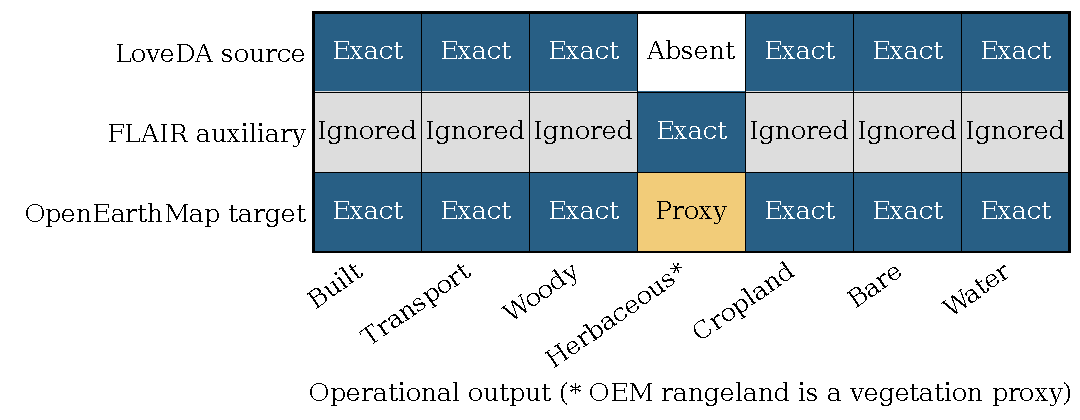
\includegraphics[width=0.92\textwidth]{fig1_coverage_20261015.pdf}
  \caption{Declared operational coverage for the primary source mixture and OpenEarthMap target. Exact means a raw label is mapped to the named common leaf under the fixed crosswalk; it does not assert universal semantic equivalence. LoveDA has no admitted source label for the herbaceous output. B1 retains FLAIR raw ID 10 and ignores all other FLAIR labels. The OEM cell marked Proxy reflects its broader rangeland definition, including shrubs (Supplementary Section S2). Semantic Drone is evaluated separately as grass versus all other pixels (Section~\ref{sec:semanticdrone_result}).}
  \label{fig:coverage}
\end{figure}

\subsection{An auxiliary FLAIR source recovers OpenEarthMap rangeland}
\label{sec:oem_result}

The largest primary contrast is concentrated in the audited missing leaf. Across the three fixed checkpoints, B0 rangeland IoU is $1.6\times10^{-7}$, 0, and 0, whereas B1 reaches 0.3124, 0.3187, and 0.3041 for seeds 19, 37, and 73. The mean paired contrast is +0.3118 with a 95\% evaluation-unit bootstrap interval of [+0.2821, +0.3399] on the Paris-excluded 74-city population (Table~\ref{tab:oem-seeds}, Figure~\ref{fig:oem-primary}). The interval resamples declared city units and is conditional on the completed checkpoints.

\begin{figure}[H]
  \centering
  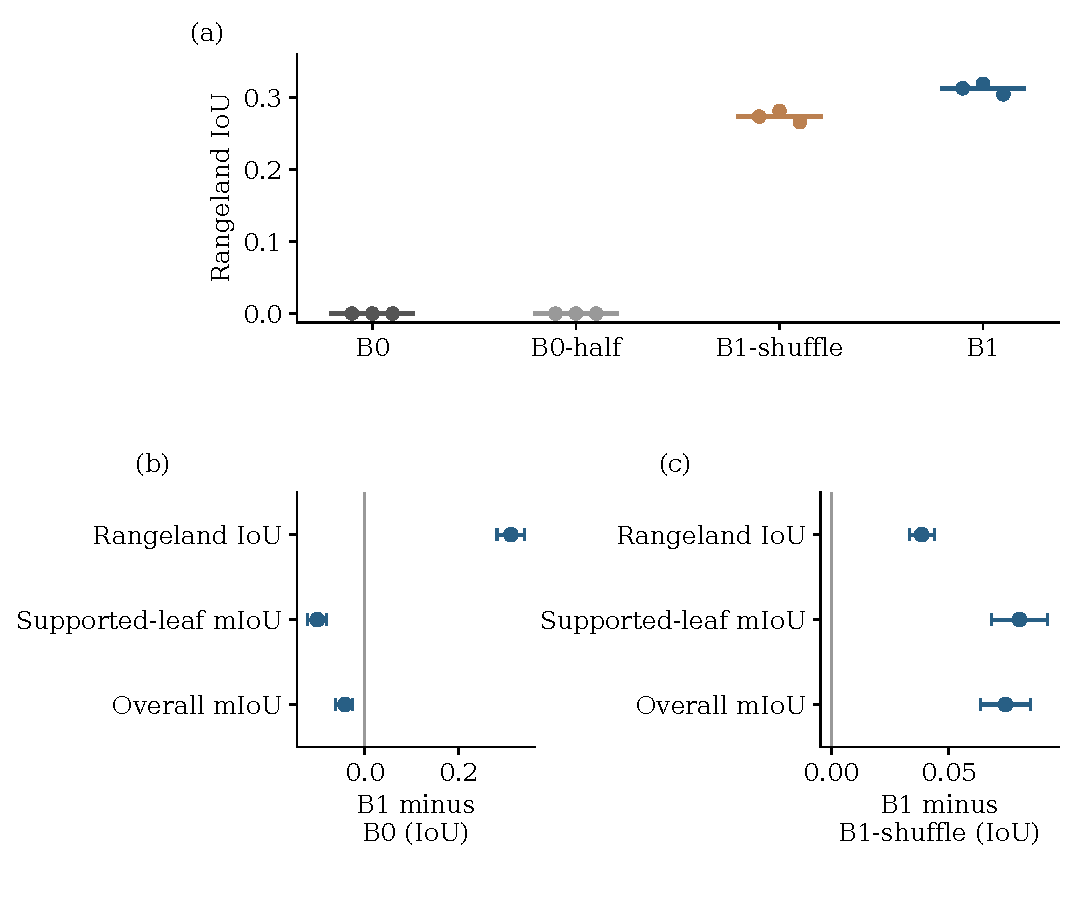
\includegraphics[width=0.92\textwidth]{fig2_oem_results_20261015.pdf}
  \caption{OpenEarthMap results on the Paris-excluded 74-city population. (a) Rangeland IoU for seeds 19, 37 and 73, with horizontal marks showing their mean; horizontal offsets separate checkpoints. (b) B1 minus B0 contrasts. (c) B1 minus the recorded B1-shuffle configuration. Panels (b) and (c) use different axis ranges and show 95\% paired city-bootstrap intervals from 2,000 draws, conditional on the three completed checkpoints. Supported-leaf mIoU averages the six LoveDA-supported leaves. Complete original shuffle schedules were not recovered: panel (c) is a configuration-based sensitivity, not a fully revalidated pairing mechanism.}
  \label{fig:oem-primary}
\end{figure}

Reduced LoveDA exposure alone does not reproduce the observed target-leaf recovery. B0-half lowers overall mIoU by 0.0069 relative to B0, while B1 retains a rangeland gain of +0.3118 after LoveDA exposure is matched (Table~\ref{tab:oem-controls}). The duplicated-crop integrity check is zero at the reported precision and is reported in Appendix Table~\ref{tab:batch_integrity}; it checks the update implementation rather than a generic batch-size effect.

\subsection{Sensitivity to the recorded pairing configuration}
\label{sec:pairing_result}

The archived B1-shuffle configuration specifies the same FLAIR image schedule and mask-density multiset with non-native masks. Full raw schedules were not recovered for independent revalidation of these constraints. It still recovers rangeland, with seedwise IoUs of 0.2732, 0.2812, and 0.2653. Its mean contrast against B0 is 0.2732, compared with 0.3118 for B1--B0. Thus, 0.2732/0.3118 = 87.6\% of the observed recovery remains in this mismatched-pair schedule, and the native B1 configuration is higher by +0.0385 (12.4\%; 95\% evaluation-unit bootstrap interval [+0.0333, +0.0439]); all three seedwise contrasts are positive. The same comparison improves overall mIoU by +0.0741 and mIoU over the six LoveDA-supported leaves by +0.0801 (Table~\ref{tab:oem-controls}). This arithmetic partition describes the specified schedules. It does not separate auxiliary image content from label support, and, because the raw primary schedules are unavailable for independent revalidation, it is reported as a configuration-based sensitivity rather than a fully verified pairing mechanism.

\begin{table}[H]
\centering
\caption{OpenEarthMap Paris-excluded 74-city replay metrics by fixed checkpoint. Values are displayed to four decimal places; the B0 rangeland IoU for seed 19 is $1.6\times10^{-7}$ and those for seeds 37 and 73 are zero. The B0 and B1 supported-leaf mIoU ranges are 0.4359--0.4468 and 0.3309--0.3473, respectively. Supported-leaf mIoU averages the six leaves with exact operational LoveDA support; it is reported beside overall mIoU rather than as an alternative overall-performance estimate. City-bootstrap contrasts are computed from unrounded checkpoint metrics and rounded only for display (Table~\ref{tab:oem-controls}).}
\label{tab:oem-seeds}
\small
\renewcommand{\arraystretch}{1.12}
\setlength{\tabcolsep}{4pt}
\begin{tabular*}{\linewidth}{@{\extracolsep{\fill}}lrrrr@{}}
\toprule
Arm & Seed & Overall mIoU & Rangeland IoU & Supported-leaf mIoU \\
\midrule
B0 & 19 & 0.3830 & 0.0000 & 0.4468 \\
B0 & 37 & 0.3802 & 0.0000 & 0.4436 \\
B0 & 73 & 0.3736 & 0.0000 & 0.4359 \\
B0-half & 19 & 0.3652 & 0.0000 & 0.4261 \\
B0-half & 37 & 0.3825 & 0.0000 & 0.4462 \\
B0-half & 73 & 0.3683 & 0.0000 & 0.4296 \\
B1-shuffle & 19 & 0.2710 & 0.2732 & 0.2707 \\
B1-shuffle & 37 & 0.2564 & 0.2812 & 0.2523 \\
B1-shuffle & 73 & 0.2604 & 0.2653 & 0.2596 \\
B1 & 19 & 0.3400 & 0.3124 & 0.3446 \\
B1 & 37 & 0.3292 & 0.3187 & 0.3309 \\
B1 & 73 & 0.3411 & 0.3041 & 0.3473 \\
\bottomrule
\end{tabular*}
\end{table}

\begin{table}[H]
\centering
\caption{Fixed-budget and shuffled-pairing OpenEarthMap control contrasts on the Paris-excluded 74-city population. Intervals are paired city-bootstrap intervals conditional on completed fixed checkpoints. Contrasts are computed from unrounded checkpoint metrics and rounded only for display. The duplicated-crop integrity check is reported in Appendix Table~\ref{tab:batch_integrity}.}
\label{tab:oem-controls}
\small
\renewcommand{\arraystretch}{1.12}
\setlength{\tabcolsep}{4pt}
\begin{tabular*}{\linewidth}{@{\extracolsep{\fill}}llrrr@{}}
\toprule
Contrast & Metric & Estimate & 95\% lower & 95\% upper \\
\midrule
B0-half $-$ B0 & overall mIoU & $-0.0069$ & $-0.0100$ & $-0.0038$ \\
B1 $-$ B0 & overall mIoU & $-0.0422$ & $-0.0613$ & $-0.0252$ \\
B1 $-$ B0 & rangeland IoU & $+0.3118$ & $+0.2821$ & $+0.3399$ \\
B1 $-$ B0-half & overall mIoU & $-0.0352$ & $-0.0538$ & $-0.0182$ \\
B1 $-$ B0-half & rangeland IoU & $+0.3118$ & $+0.2821$ & $+0.3399$ \\
B1 $-$ B0 & supported-leaf mIoU & $-0.1011$ & $-0.1213$ & $-0.0821$ \\
B1 $-$ B0-half & supported-leaf mIoU & $-0.0931$ & $-0.1128$ & $-0.0741$ \\
B1 $-$ B1-shuffle & overall mIoU & $+0.0741$ & $+0.0634$ & $+0.0848$ \\
B1 $-$ B1-shuffle & supported-leaf mIoU & $+0.0801$ & $+0.0682$ & $+0.0921$ \\
B1 $-$ B1-shuffle & rangeland IoU & $+0.0385$ & $+0.0333$ & $+0.0439$ \\
\bottomrule
\end{tabular*}
\end{table}


\subsection{Recovery is accompanied by a supported-leaf trade-off}
\label{sec:tradeoff_result}

The target-leaf gain does not improve the full operating profile. B1 mean mIoU is 0.3368 compared with 0.3789 for B0, while mIoU over the six leaves with exact operational LoveDA support changes by -0.1011 (95\% evaluation-unit bootstrap interval [-0.1213, -0.0821]). The two metrics answer different questions: overall mIoU includes the recovered rangeland leaf, whereas the defined supported-leaf metric excludes it to report the retained LoveDA leaves. Their numerical differences are therefore not competing effect-size estimates. The seed-level supported-leaf mIoU ranges from 0.4359 to 0.4468 for B0 and from 0.3309 to 0.3473 for B1 (Table~\ref{tab:oem-seeds}); inference remains the declared city-unit bootstrap, not a three-seed test. Matching LoveDA exposure leaves a supported-leaf contrast of -0.0931 for B1--B0-half (Table~\ref{tab:oem-controls}). Figure~\ref{fig:oem-tradeoff} shows the leafwise pattern: rangeland is recovered, whereas the largest observed supported-leaf decline is cropland. Complete unadjusted descriptive intervals are reported in Appendix Table~\ref{tab:all_leaf_contrasts}.

\begin{figure}[H]
  \centering
  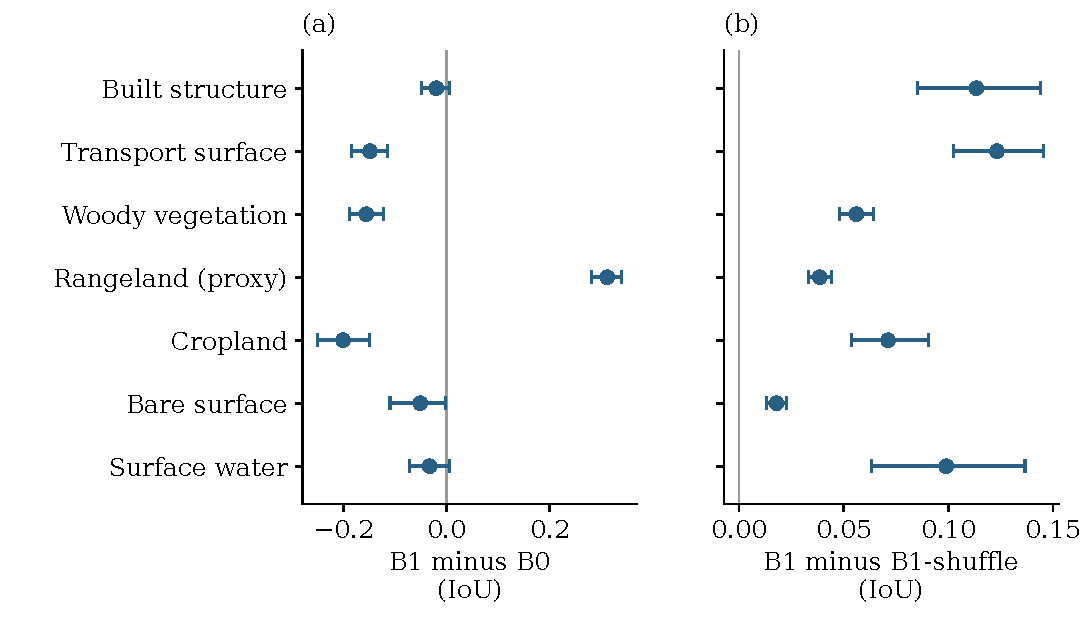
\includegraphics[width=0.92\textwidth]{fig3_leaf_contrasts_20261015.pdf}
  \caption{Leafwise OpenEarthMap contrasts on the Paris-excluded 74-city population. (a) B1 minus B0; (b) B1 minus the recorded B1-shuffle configuration. Both panels use the same seven leaf rows and report 95\% descriptive paired city-bootstrap intervals from 2,000 draws, conditional on checkpoints 19, 37 and 73. Panel (b) is a configuration-based sensitivity: complete original shuffle schedules were not recovered for independent revalidation of pairing and exposure constraints. The two panels use different horizontal scales.}
  \label{fig:oem-tradeoff}
\end{figure}

\subsection{The archived native U-Net comparison repeats the direction}
\label{sec:unet_result}
Across the three archived native U-Net checkpoints, U-B0 and U-B0-half both give zero rangeland IoU. U-B1 gives 0.2957, 0.2767 and 0.2762, with mean 0.2828 and sample SD 0.0111. The U-B1--U-B0 contrast is +0.2828 (95\% checkpoint-conditional paired city interval [+0.2512, +0.3133]). Supported-leaf mIoU changes from 0.2329 to 0.1025, a contrast of -0.1304 (interval [-0.1529, -0.1075]); against U-B0-half it changes by -0.1182 (interval [-0.1390, -0.0965]). Every matched seed has positive rangeland recovery and lower supported-leaf mIoU for both native baseline comparisons (Table~\ref{tab:unet-native}).

The archived evaluation records therefore show recovery with retention loss in a second recorded architecture on the common target. They do not supply an independent target population, a pure-label causal experiment or a CLIP--U-Net superiority comparison. Original checkpoint, spatial reference and historical-code provenance limits remain as specified in Section~\ref{sec:unet_protocol}. Shuffled U-Net results do not enter this conclusion.

\begin{table}[H]
\centering
\caption{Archived native U-Net comparison on the same Paris-excluded 74-city OpenEarthMap target (2,638 rasters). Means and sample SDs summarize the three recorded seed checkpoints; SDs are descriptive. Contrasts use 2,000 paired city draws and 95\% intervals conditional on the fixed recorded checkpoints, not training-seed uncertainty. Supported-leaf mIoU averages the six LoveDA-supported leaves. U-B0-half matches LoveDA exposure in U-B1. Original checkpoint and spatial reference bytes were not replayed; this is a within-family archived-record comparison.}
\label{tab:unet-native}
\small
\setlength{\tabcolsep}{3pt}
\begin{tabular*}{\linewidth}{@{\extracolsep{\fill}}lrrr@{}}
\toprule
Arm & Rangeland IoU & Supported-leaf mIoU & Overall mIoU \\
\midrule
U-B0 & $0.0000 \pm 0.0000$ & $0.2329 \pm 0.0158$ & $0.1996 \pm 0.0136$ \\
U-B0-half & $0.0000 \pm 0.0000$ & $0.2207 \pm 0.0261$ & $0.1892 \pm 0.0223$ \\
U-B1 & $0.2828 \pm 0.0111$ & $0.1025 \pm 0.0209$ & $0.1283 \pm 0.0190$ \\
\bottomrule
\end{tabular*}
\par\medskip
\begin{tabular*}{\linewidth}{@{\extracolsep{\fill}}lrrr@{}}
\toprule
Contrast and metric & Estimate & 95\% lower & 95\% upper \\
\midrule
U-B1 $-$ U-B0 / rangeland & $+0.2828$ & $+0.2512$ & $+0.3133$ \\
U-B1 $-$ U-B0 / supported & $-0.1304$ & $-0.1529$ & $-0.1075$ \\
U-B1 $-$ U-B0-half / rangeland & $+0.2828$ & $+0.2512$ & $+0.3133$ \\
U-B1 $-$ U-B0-half / supported & $-0.1182$ & $-0.1390$ & $-0.0965$ \\
\bottomrule
\end{tabular*}
\end{table}


\subsection{Second target evaluation on Semantic Drone}
\label{sec:semanticdrone_result}

On the primary 400-raster evaluation, frozen E0 gives grass IoU 0.0224, whereas each of the three LoveDA-only B0 checkpoints gives 0.0000. The three B1 checkpoints give 0.2282, 0.2305, and 0.2228 (mean 0.2272; sample SD 0.0040). The descriptive mean B1--B0 contrast is +0.2272 (Supplementary Sections S9 and S11). No three-checkpoint raster-resampling interval is claimed in this revision. The E0-to-B0 decline is a checkpoint diagnostic consistent with LoveDA-only calibration suppressing the limited grass score present in the frozen probe; it does not identify the mechanism. This is a second-target evaluation of the primary source mixture, not a model-level replication: it reuses the probe, prompts, and training budget. The archived record identifies the target manifest and source-archive hashes; independently timestamped pre-inference provenance is not established here.





\subsection{A second source mixture shows the same recovery--trade-off direction}
\label{sec:second_mixture_result}

The source-role-reversed case begins with a different audited gap: Semantic Drone has no exact operational cropland label, whereas LoveDA agriculture and OpenEarthMap \texttt{agriculture\_land} provide declared cropland support. On the frozen 72-city OpenEarthMap population, SD-B0 and the exposure-matched SD-B0-half produce cropland IoU of zero for every seed. SD-B1 reaches 0.1627, 0.1642, and 0.1627, giving a mean paired SD-B1--SD-B0 difference of +0.1632 (95\% evaluation-unit bootstrap interval: [+0.1262, +0.2049]; Table~\ref{tab:second-mixture}).

The recovery again carries a fixed-budget cost. Over the three leaves with exact operational Semantic Drone support, SD-B1 changes base-source mIoU by -0.1686 relative to SD-B0 (95\% evaluation-unit bootstrap interval [-0.1903, -0.1464]) and by -0.1337 relative to exposure-matched SD-B0-half (interval [-0.1534, -0.1151]). The planned shuffled auxiliary-mask arm met multiset and no-native-pair constraints, but its post-run schedule audit found per-pair density mismatches and retired the contrast. Its efficacy is not interpreted. This case tests a second audited source mixture, not a second pairing-control result or an independent target-pair replication.

\begin{table}[H]
\centering
\caption{Second source-mixture replay: Semantic Drone as the base source, LoveDA agriculture as an auxiliary source supplying cropland supervision, and OpenEarthMap as the target. The base-source metric averages the three leaves with exact operational Semantic Drone support: herbaceous vegetation, woody vegetation, and surface water. Point values average three completed checkpoints. Contrasts are computed from unrounded checkpoint metrics and rounded only for display. Intervals are paired 2,000-draw city-bootstrap intervals conditioned on those checkpoints and the 72-city target population excluding Shanghai, Tyrol, and Vienna.}
\label{tab:second-mixture}
\small
\renewcommand{\arraystretch}{1.12}
\setlength{\tabcolsep}{4pt}
\begin{tabular*}{\linewidth}{@{\extracolsep{\fill}}lrrrr@{}}
\toprule
\multicolumn{5}{l}{Cropland IoU by checkpoint and its mean} \\
Arm & Seed 19 & Seed 37 & Seed 73 & Mean \\
\midrule
SD-B0 & 0.0000 & 0.0000 & 0.0000 & 0.0000 \\
SD-B0-half & 0.0000 & 0.0000 & 0.0000 & 0.0000 \\
SD-B1 & 0.1627 & 0.1642 & 0.1627 & 0.1632 \\
\bottomrule
\end{tabular*}
\par\medskip
\begin{tabular*}{\linewidth}{@{\extracolsep{\fill}}lrl@{}}
\toprule
Arm & Base-source mIoU & Role \\
\midrule
SD-B0 & 0.2686 & Base source \\
SD-B0-half & 0.2337 & Exposure control \\
SD-B1 & 0.1001 & Auxiliary cropland source \\
\bottomrule
\end{tabular*}
\par\medskip
\begin{tabular*}{\linewidth}{@{\extracolsep{\fill}}lrrr@{}}
\toprule
SD-B1 minus SD-B0 & Estimate & 95\% lower & 95\% upper \\
\midrule
Cropland IoU & +0.1632 & +0.1262 & +0.2049 \\
Base-source mIoU & -0.1686 & -0.1903 & -0.1464 \\
\bottomrule
\end{tabular*}
\par\smallskip
\raggedright All three checkpoint-specific cropland contrasts are positive.
\end{table}


The separate B2 learnability diagnostic is reported in Supplementary Sections S8 and S11. They do not select or alter the primary source-mixture endpoints.

\section{Discussion}
\label{sec:discussion}
\subsection{An empirical diagnostic within an established problem}
Legend compatibility, heterogeneous annotations and class-space differences are established concerns \citep{yang2017harmonization,lambert2020mseg,kim2022uniseg}. Transferable land-cover semantics are also studied by TACOSS and LandSegmenter \citep{zermatten2025tacoss,liu2026landsegmenter}. The present contribution is a bounded empirical audit: connect the declared crosswalk to the masks actually available to a particular learner, then report the tested source mixture's recovery and supported-leaf cost under the specified controls. Neither taxonomy construction nor negative transfer is claimed as a new discovery.

Exact-label absence qualifies the available supervision; it does not exclude visual shift, establish a sole cause of failure or imply that a pretrained or heterogeneous-supervision model cannot recognize the concept. The primary CLIP and archived native U-Net comparisons show the same direction under their respective recorded training regimes. That extension narrows an explanation restricted to this one CLIP calibration instrument, but two chosen model families on a shared target do not establish architecture-wide generality.

\subsection{What source mixtures and pairing establish}
The primary experiment adds FLAIR imagery and herbaceous labels together. Exposure and duplicate-crop controls constrain two alternative explanations but do not turn that contrast into a label-only intervention. The recorded mismatched configuration retains most recovery, and native B1 gives a smaller additional contrast. Missing complete primary schedule files limit independent verification of pairing and exposure constraints. Auxiliary image content, regional statistics and weak alignment under same-region derangement remain compatible explanations. The retained recovery fraction is an arithmetic description, not a causal percentage attributable to a component. The retired U-Net and reversed-source shuffle arms provide no further efficacy claim.

A missing-leaf gain does not establish better aggregate transfer or preserved prior capabilities. Common/private performance reporting and known-class negative transfer already appear in adaptation research \citep{choe2024bus,choe2025unida,ren2026sats}. Here, the reported costs concern six exact LoveDA-supported leaves, or the three exact Semantic Drone-supported leaves in the reversed case. Decision-boundary changes, source appearance, sampling and loss weighting remain possible contributors. The experiments do not identify representational capacity as the cause and do not validate a mitigation module.

\subsection{Replication and provenance boundaries}
Semantic Drone supplies a second target replay using the primary CLIP checkpoints; its grass-versus-rest metric does not measure retention over all supported leaves. The reversed source-mixture case changes the missing leaf but reuses the OpenEarthMap target release. The native U-Net records change the architecture but retain the primary target population. These extensions are complementary checks with shared components, not a fully independent architecture-by-target replication. B2 establishes learnability under a different direct-supervision regime, not external-transfer superiority.

Semantic Drone's three-checkpoint points are reconstructable from archived integer totals, but per-raster records for two checkpoints were not recovered; its archived multi-checkpoint interval is not used. Native U-Net identifier sets and per-raster reference marginals match the primary population, but spatial label equality and original checkpoint execution are not thereby verified. The source-ready audit content is recovered by hash; this does not recover historical timestamp or executed-code identity. City/raster intervals condition on recorded checkpoints, not training-seed uncertainty or independent geographic sites. Geographic guards reduce named overlap risks without proving coordinate-level separation. Within these limits, a deployment report can make both the tested missing-leaf gain and its source-supported cost explicit.


\subsection{Class-proxy and construct-validity boundary}
The fixed codebook does not make the native annotation meanings identical. OEM rangeland includes bushes and shrubs, so its assignment to the herbaceous output is a coarse vegetation proxy (Supplementary Section S2). The reported rangeland recovery remains a native-label score under that declared mapping; it is not evidence of recovery restricted to pure herbaceous pixels. No grass/shrub subdivision is available in the retained OEM reference labels. Consequently, ontology resolution and annotation scope remain plausible contributors alongside imagery and supervision. We retain the original mappings, prompts, checkpoints and integer scores and do not synthesize a botanical reference or change model selection to resolve this limitation.

\section{Conclusion}
\label{sec:conclusion}
Raw-mask audits under the declared operational crosswalk show that the primary LoveDA source lacks exact herbaceous supervision. With the specified CLIP probe and update budget, adding the tested FLAIR source mixture recovers OpenEarthMap rangeland while reducing performance on source-supported leaves. Archived native U-Net records repeat that direction on the same target; a second target replay and a reversed source mixture extend the descriptive evidence within their stated dependence and provenance limits. These findings add a concrete audit and controlled empirical analysis to established label-space and negative-transfer research. Positive source-label coverage, missing-leaf recovery and supported-leaf retention should be reported together. The experiments neither isolate a label-only causal effect nor establish a solution to the trade-off.

\section*{Disclosures}
The authors declare no conflicts of interest related to this work.

\section*{Code and Data Availability}
LoveDA, FLAIR, OpenEarthMap and Semantic Drone are available from their original providers cited in the text, subject to the providers' terms. Provider imagery and spatial masks are not redistributed in the local review package. The prepared local code-and-results package contains analysis scripts, ontology mappings, raw-label audit records, run configurations, identifier/reference-count records, retained integer confusions, and a SHA256 manifest. A separate local checkpoint archive contains the nine recovered native ResNet-34 U-Net checkpoints; each matches the checkpoint digest recorded in its original evaluation configuration. These byte checks do not constitute model inference replay or verification of historical initialization, spatial-mask identity or executed-code provenance. The complete primary pairing schedules and two Semantic Drone per-checkpoint raster records remain unavailable in the searched materials; related claims and intervals are restricted accordingly. Code and retained analysis records are available at \url{https://github.com/Loquat-0813/landcover-transfer-audit}. The repository documents its file inventory, verification commands and evidence limitations. Provider datasets and model checkpoints are not redistributed in the repository. A persistent archival identifier has not been assigned.

\section*{Acknowledgments}
This work was supported by the Natural Science Foundation of Fujian Province (Grant No. 2026J001311) and the China Scholarship Council (Grant No. 2023063508). OpenAI Codex assisted with code drafting, literature discovery, organization and recomputation of retained experimental records, figure and table preparation, and manuscript drafting and revision. The named authors are responsible for checking and approving all scientific statements and the final manuscript. Specific uses are described in Section~\ref{sec:ai_assistance}.


\bibliographystyle{spiejour}
\bibliography{references}

\clearpage
\appendix
\renewcommand{\thetable}{A.\arabic{table}}
\setcounter{table}{0}
\section{Reproducibility and integrity conditions}
\label{app:integrity}

The frozen ontology contains seven leaves: built structure, transport surface, woody vegetation, herbaceous vegetation, cropland, bare surface, and surface water. Herbaceous vegetation is the frozen output-index name; its OEM target relation is the broader rangeland vegetation proxy, including bushes/shrubs, while the Semantic Drone relation is grass. These output aliases do not define a fully reconciled botanical taxonomy. Cropland denotes the declared agricultural-field or managed-cover relation. Under the frozen crosswalk, LoveDA building, road, forest, agriculture, barren, and water provide exact operational support for six non-herbaceous leaves. FLAIR raw ID 10 is the only FLAIR label admitted by B1. OpenEarthMap rangeland and Semantic Drone grass are declared target relations. OpenEarthMap developed space remains a coarser ancestor, not building or road support.

\begin{table}[h]
\centering
\caption{Complete frozen prompt set used by every reported arm.}
\label{tab:prompts}
\begin{tabular}{ll}
\toprule
Common leaf & Prompt \\
\midrule
Built structure & a satellite image of a building \\
Transport surface & a satellite image of a road \\
Woody vegetation & a satellite image of forest or trees \\
Herbaceous vegetation & a satellite image of grassland or rangeland \\
Cropland & a satellite image of agricultural cropland \\
Bare surface & a satellite image of bare soil or barren ground \\
Surface water & a satellite image of water \\
\bottomrule
\end{tabular}
\end{table}

Each raster is partitioned at stride 512 into non-overlapping \(512\times512\) RGB tiles. Only the right and bottom edge tiles are zero-padded. CLIP patch features are scored, logits are bilinearly interpolated to \(512\times512\) with the align-corners parameter set to false, and the leaf argmax is copied over the unpadded tile extent. No overlap, blending, test-time augmentation, or post-processing is used.

For B0-half-batch2, duplicate copies of the same deterministic crop have the same individual loss. With mean loss, a frozen backbone, no train-mode batch-dependent state, no sample-dependent random transformation at the adapter, and identical optimizer state, the mean gradient equals the one-crop gradient at every update. The absolute mean-mIoU contrast is below \(4\times10^{-9}\), numerically zero at the reported precision; it is therefore a constructive pipeline-integrity check, not an empirical estimate of a generic batch-size effect.

\begin{table}[h]
\centering
\caption{Duplicated-crop pipeline-integrity check. B0-half-batch2 duplicates the deterministic LoveDA crop in the second update slot.}
\label{tab:batch_integrity}
\begin{tabular}{@{}p{0.28\linewidth}p{0.30\linewidth}p{0.27\linewidth}@{}}
\toprule
Contrast & Metric & Audited result \\
\midrule
B0-half-batch2 minus B0-half & absolute mean mIoU difference & below \(4\times10^{-9}\) \\
\bottomrule
\end{tabular}
\end{table}

Table~\ref{tab:all_leaf_contrasts} provides the complete descriptive, unadjusted intervals for the seven OpenEarthMap leaves.

\begin{table}[h]
\centering
\caption{Unadjusted descriptive paired city-bootstrap intervals for all OpenEarthMap leaf contrasts. The primary target leaf is herbaceous/rangeland.}
\label{tab:all_leaf_contrasts}
\begin{tabular}{lrrr}
\toprule
Leaf & B1 minus B0 IoU & Lower & Upper \\
\midrule
Built structure & -0.01958 & -0.04881 & +0.00555 \\
Transport surface & -0.1482 & -0.1845 & -0.1134 \\
Woody vegetation & -0.1554 & -0.1880 & -0.1225 \\
Rangeland proxy & +0.3118 & +0.2821 & +0.3399 \\
Cropland & -0.2005 & -0.2497 & -0.1498 \\
Bare surface & -0.05080 & -0.1094 & -0.00103 \\
Surface water & -0.03249 & -0.07099 & +0.00676 \\
\bottomrule
\end{tabular}
\end{table}

\end{spacing}
\end{document}
